\documentclass{article}
\usepackage{graphicx}
\graphicspath{ {./Pictures/} }
\usepackage[table,xcdraw]{xcolor}

\title{\textbf{Chapter}}
\author
{\underline{Urszula Kostuch}}
\date{03 November 2022}

\begin{document}

\maketitle

\section{Math}
The formula of quadratic function:
\[f(x)=ax^2+bx+c\]
Another frequently used equation:
\[\sin^2(\alpha) +\cos^2(\alpha) =1\]
I live in {\textbf{Cracow}}. This city is one of the \undeline{most beautiful} cities I have \textbf{ever seen.} Cracow, is the second-largest and one of the oldest cities in Poland. \underline{Situated on the Vistula River in Lesser Poland Voivodeship.}  \textbf{Cited as one of Europe's most beautiful cities, its Old Town with Wawel Royal Castle was declared the first UNESCO World Heritage Site in the world.}

\begin{figure}[h!]
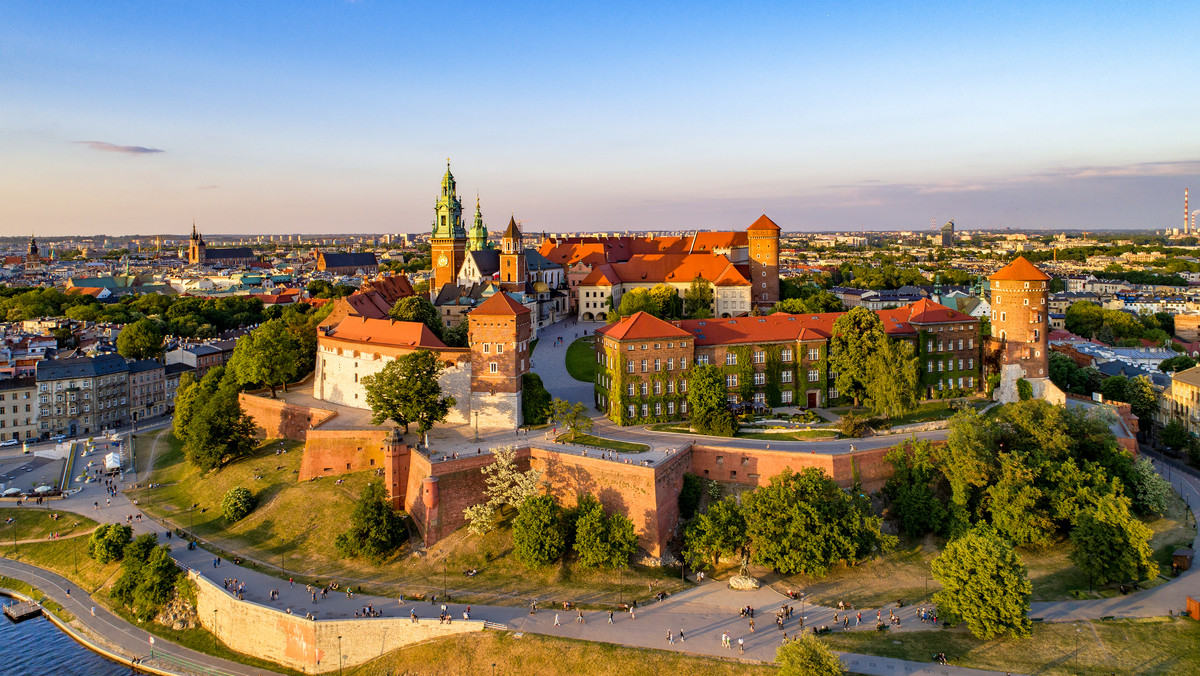
\includegraphics[width=\linewidth]{Pictures/wawel.jpg}
\caption{Zamek krolewski na Wawelu}
  \label{fig:wawel}
\end{figure}
\pagebreak
\section{Must-see places in Cracow:}
\centering
\begin{itemize}
  \item \textit{Sukiennice
  \item Wawel
  \item Kazimierz}
\end{itemize}
\begin{enumerate}
  \item Blonie
  \item Bulwary
  \item Park Jordana
\end{enumerate}

\begin{table}[]
\begin{tabular}{|l|l|l|l|l|}
\hline
\rowcolor[HTML]{9AEAEA} 
\cellcolor[HTML]{E1BCF9}1 & 1 & 2 & 3 & 4 \\ \hline
\cellcolor[HTML]{E1BCF9}2 & 2 & 4 & 6 & 8 \\ \hline
\cellcolor[HTML]{E1BCF9}3 & 3 & 6 & 9 & 12 \\ \hline
\cellcolor[HTML]{E1BCF9}4 & 4 & 8 & 12 & 16 \\ \hline
\end{tabular}
\caption{Table to test}
\label{table:1}
\end{table}

\end{document}